\newpage
\section{Các mô hình tương tự CLIP}

\subsection{ALIGN} 

\paragraph{}{Trong phương pháp \textbf{ALIGN} được giới thiệu trong bài báo \textbf{Scaling Up Visual and Vision-Language Representation Learning With Noisy Text Supervision} \cite{jia2021scalingvisualvisionlanguagerepresentation}, các biểu diễn (representations) hình ảnh và ngôn ngữ được huấn luyện đồng thời từ dữ liệu nhiễu (noisy) là các cặp ảnh và văn bản thay thế (alt-text). Các bộ mã hóa hình ảnh (image encoder) và văn bản (text encoder) được học thông qua hàm mất mát tương phản (contrastive loss), được định dạng dưới dạng softmax chuẩn hóa. Hàm mất mát này có tác dụng đẩy các embedding của cặp ảnh-văn bản khớp nhau lại gần nhau hơn, đồng thời đẩy chúng ra xa các embedding của những cặp ảnh-văn bản không khớp.\\

% Mô hình học cách căn chỉnh (align) các biểu diễn hình ảnh và ngôn ngữ của các cặp ảnh-văn bản bằng cách sử dụng hàm mất mát tương phản. Các biểu diễn này có thể được sử dụng để chuyển giao cho các tác vụ chỉ liên quan đến thị giác (vision-only) hoặc các tác vụ ngôn ngữ-thị giác (vision-language). Không cần bất kỳ tinh chỉnh (fine-tuning) nào, ALIGN có thể thực hiện phân loại hình ảnh zero-shot và tìm kiếm chéo phương thức (cross-modal search), bao gồm tìm kiếm từ ảnh sang văn bản, từ văn bản sang ảnh, và thậm chí tìm kiếm với các truy vấn kết hợp cả ảnh và văn bản.
}

\begin{figure}[H]
    \centering
    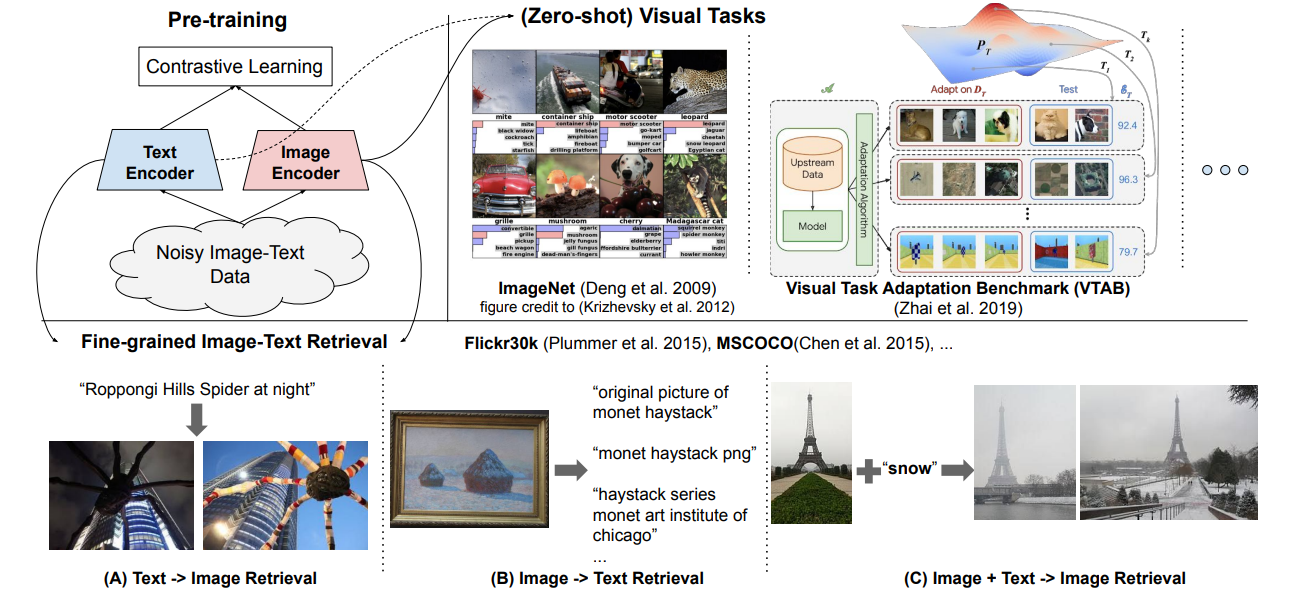
\includegraphics[width=1\linewidth]{img/06-ALIGN.png}
    \caption{Tóm tắt phương pháp ALIGN.}
\end{figure}

\paragraph{}{\textbf{Mục tiêu chính:} Mục tiêu của ALIGN là học các biểu diễn (representations) mạnh mẽ cho cả thị giác (vision) và ngôn ngữ-thị giác (vision-language) bằng cách mở rộng quy mô dữ liệu huấn luyện lên mức cực lớn, nhưng với một phương pháp thu thập dữ liệu đơn giản, ít tốn kém. Giả thuyết cốt lõi của họ là \textbf{quy mô của dữ liệu có thể bù đắp cho sự nhiễu} của nó.}

\paragraph{}{\textbf{Kĩ thuật chính:}}

\begin{itemize}
    \item \textbf{Dữ liệu (Data)}: Đây là điểm đột phá và khác biệt nhất của ALIGN. 
    \begin{itemize}
        \item \textbf{Nguồn}: Họ sử dụng một tập dữ liệu khổng lồ gồm hơn 1.8 tỷ cặp ảnh và alt-text (văn bản thay thế cho ảnh) được thu thập từ web.

        \item \textbf{Đặc điểm}: Dữ liệu này rất "nhiễu" (noisy). Các alt-text thường không phải là mô tả hoàn hảo, có thể chứa thông tin không liên quan, tên file, hoặc chỉ là một vài từ khóa.

        \item \textbf{Quy trình lọc}: Thay vì áp dụng các bước lọc và xử lý phức tạp, tốn kém như các bộ dữ liệu được giám sát kỹ lưỡng (ví dụ: Conceptual Captions), ALIGN chỉ áp dụng các bộ lọc rất đơn giản dựa trên tần suất (frequency-based filtering). Ví dụ: loại bỏ các ảnh/văn bản khiêu dâm, ảnh có kích thước quá nhỏ, hoặc các alt-text quá phổ biến (như "ảnh"), quá ngắn hoặc quá dài.
    \end{itemize}

    \item \textbf{Kiến trúc mô hình (Model architecture)}:
    \begin{itemize}
        \item ALIGN sử dụng một kiến trúc \textbf{bộ mã hóa kép (dual-encoder)}.

        \item \textbf{Image Encoder}: Một mạng CNN, cụ thể là \textbf{EfficientNet}.

        \item \textbf{Text Encoder}: Một mạng Transformer, cụ thể là \textbf{BERT}.

        \item Kiến trúc này lấy một ảnh và một đoạn văn bản, mã hóa chúng một cách độc lập để tạo ra hai vector embedding.
    \end{itemize}

    \item \textbf{Hàm mục tiêu (Loss function)}:
    \begin{itemize}
        \item Cả Image encoder và Text encoder được huấn luyện bằng một \textbf{hàm mất mát tương phản (contrastive loss)}, cụ thể là normalized softmax loss (còn gọi là InfoNCE).
        \item \textbf{Cách hoạt động}: Trong một batch dữ liệu, với mỗi cặp (ảnh, văn bản) đúng, mô hình sẽ cố gắng kéo vector embedding của chúng lại gần nhau trong không gian biểu diễn chung. Đồng thời, nó sẽ đẩy embedding của cặp đó ra xa khỏi tất cả các embedding của các ảnh và văn bản khác trong batch (được coi là các cặp "âm" - negative pairs). Quá trình này giúp "căn chỉnh" (align) không gian biểu diễn của ảnh và văn bản.
    \end{itemize}

\end{itemize}

\subsection{BLIP}
\paragraph{}{BLIP được giới thiệu trong bài báo \textbf{BLIP: Bootstrapping Language-Image Pre-training for Unified Vision-Language Understanding and Generation} \cite{li2022blipbootstrappinglanguageimagepretraining}. Các mô hình tiền huấn luyện thị giác-ngôn ngữ (Vision-Language Pre-training, viết tắt là VLP) đã nâng cao hiệu suất cho nhiều tác vụ thị giác-ngôn ngữ. Tuy nhiên, hầu hết VLP chỉ vượt trội ở một trong hai tác vụ: \textbf{hiểu} (understanding) hoặc \textbf{sinh} (generation). BLIP là mô hình có thể làm tốt ở cả hai nhiệm vụ này. BLIP còn có phiên bải cải tiến là BLIP-2 \cite{li2023blip2bootstrappinglanguageimagepretraining}.}

\paragraph{}{\textbf{Mục tiêu chính:}}

\begin{itemize}
    \item \textbf{Về mô hình:} Các mô hình hiện có thường chỉ xuất sắc ở một trong hai loại tác vụ: hoặc là các tác vụ \textbf{hiểu} (understanding) như truy xuất ảnh, phân loại (dựa trên kiến trúc encoder), hoặc là các tác vụ \textbf{sinh} (generation) như tạo chú thích ảnh (dựa trên kiến trúc encoder-decoder). BLIP muốn tạo ra một mô hình \textbf{thống nhất (unified)} có thể làm tốt cả hai.
    \item \textbf{Về dữ liệu:} Các mô hình như ALIGN và CLIP đạt được thành công bằng cách tăng quy mô dữ liệu với các cặp (ảnh, alt-text) nhiễu từ web. BLIP cho rằng đây chưa phải là cách tối ưu và đề xuất một phương pháp \textbf{chủ động cải thiện chất lượng dữ liệu} thay vì chỉ chấp nhận sự nhiễu loạn của nó.
\end{itemize}

\begin{figure}[H]
    \centering
    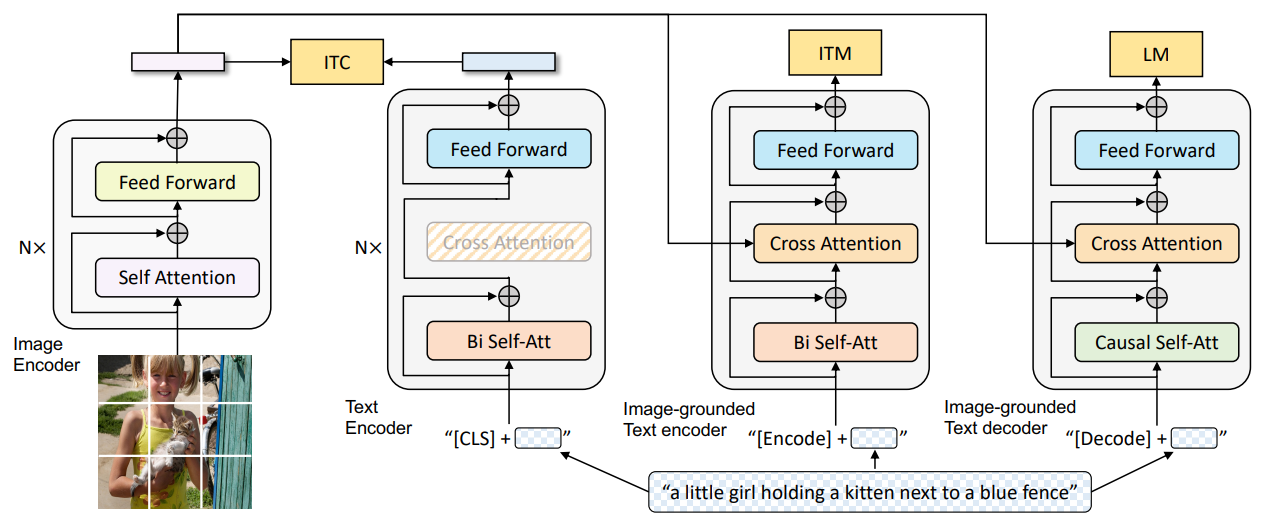
\includegraphics[width=1\linewidth]{img/06-BLIP.png}
    \caption{Tổng quan mô hình BLIP}
\end{figure}

\paragraph{}{\textbf{Kỹ thuật chính:} BLIP giới thiệu hai đóng góp chính - về dữ liệu và về kiến trúc mô hình.}

\begin{itemize}
    \item \textbf{CapFilt (Captioning and Filtering) - Tự cải thiện dữ liệu:} Đây là ý tưởng đột phá nhất của BLIP, một quy trình "bootstrapping" để làm sạch và làm giàu dữ liệu.
    \begin{enumerate}
        \item \textbf{Huấn luyện mô hình ban đầu:} Đầu tiên, họ huấn luyện một mô hình BLIP cơ bản trên 14 triệu cặp ảnh-văn bản nhiễu từ web.
        \item \textbf{Tạo hai mô-đun chuyên dụng:} Từ mô hình đã huấn luyện, họ tinh chỉnh (fine-tune) để tạo ra hai mô-đun: 
        \begin{itemize}
            \item \textbf{Captioner} (Bộ tạo chú thích): Một bộ giải mã (decoder) có khả năng tạo ra các chú thích mới (synthetic captions) cho các ảnh trên web.
            \item \textbf{Filter} (Bộ lọc): Một bộ mã hóa (encoder) học cách xác định xem một cặp (ảnh, văn bản) có khớp nhau hay không.
        \end{itemize}
        \item \textbf{Cải thiện dữ liệu:}
        \begin{itemize}
            \item \textbf{Sinh chú thích mới:} Dùng Captioner để tạo một chú thích mới cho mỗi ảnh từ web.
            \item \textbf{Lọc nhiễu:} Dùng Filter để loại bỏ những cặp (ảnh, văn bản) không khớp. Quá trình lọc này được áp dụng cho cả chú thích gốc từ web và chú thích mới được tạo ra.
        \end{itemize}
        \item \textbf{Huấn luyện mô hình cuối cùng}: Họ kết hợp tập dữ liệu đã được làm sạch và làm giàu này với các bộ dữ liệu chất lượng cao có sẵn (như COCO) để huấn luyện một mô hình BLIP mới từ đầu.
    \end{enumerate}

    Kết quả là họ có một tập dữ liệu huấn luyện lớn, vừa sạch hơn, vừa đa dạng hơn về mặt ngữ nghĩa.

    \item \textbf{MED (Multimodal Mixture of Encoder-Decoder) - Kiến trúc thống nhất:} Để phục vụ cả tác vụ hiểu và sinh, BLIP đề xuất một kiến trúc đa năng có thể hoạt động ở ba chế độ:
    \begin{enumerate}
        \item \textbf{Encoder đơn phương thức (Unimodal Encoder)}: Hoạt động như ALIGN/CLIP. Mã hóa ảnh và văn bản một cách riêng biệt, sau đó dùng contrastive loss (ITC) để căn chỉnh chúng. Dùng cho tác vụ truy xuất.
        \item \textbf{Bộ mã hóa văn bản dựa trên ảnh (Image-grounded Text Encoder)}: Thêm các lớp chú ý chéo (cross-attention) để kết hợp thông tin hình ảnh vào biểu diễn văn bản. Dùng hàm loss image-text matching (ITM) để học sự tương hợp ở mức độ chi tiết hơn (xác định cặp ảnh-văn bản là "positive" hay "negative"). Dùng cho tác vụ hiểu sâu hơn.
        \item \textbf{Bộ giải mã văn bản dựa trên ảnh (Image-grounded Text Decoder)}: Sử dụng các lớp tự chú ý nhân quả (causal self-attention) để sinh văn bản dựa trên ảnh đầu vào. Dùng hàm loss Language Modeling (LM). Dùng cho tác vụ sinh văn bản như tạo chú thích, trả lời câu hỏi.
        
    \end{enumerate}

    Kiến trúc này rất thông minh ở chỗ nó chia sẻ phần lớn các tham số giữa ba chế độ, giúp việc huấn luyện hiệu quả.
\end{itemize}

\subsection{So sánh CLIP, ALIGN và BLIP}

\begin{table}[H]
{%
\begin{tabular}{|l|p{4.5cm}|p{4.5cm}|p{4.5cm}|}
\hline
\textbf{Tính năng} & \textbf{ALIGN (Google)} & \textbf{CLIP (OpenAI)} & \textbf{BLIP (Salesforce)} \\ \hline
Triết lý & Quy mô dữ liệu bù đắp sự nhiễu & Đặt nền móng cho các tác vụ zero-shot. & Linh hoạt, hiểu sâu ảnh-văn bản. \\ \hline
Kiến trúc & EfficientNet - BERT. & Resnet/ViT-Transformer & MED \\ \hline
Dữ liệu & 1.8 tỷ cặp ảnh-văn bản thô từ web. & 400 triệu cặp ảnh-văn bản (WIT). & Tự tạo và lọc dữ liệu (CapFilt). \\ \hline
Thế mạnh & - NLP đa dạng. \newline - Truy vấn rộng& - Phân loại Zero-shot. \newline - Retrieval image. & - Image captioning. \newline - VQA. \\ \hline
Ứng dụng & Hệ thống tìm kiếm hình ảnh bằng ngôn ngữ tự nhiên, phức tạp. & Tác vụ phân loại nhanh mà không cần fine-tuning. & Ứng dụng đòi hỏi sự hiểu biết chi tiết hình ảnh-văn bản. \\ \hline
\end{tabular}%
}
\end{table}


